\documentclass[tikz,border=10pt]{standalone}
\usepackage{amsmath}
\usepackage{amssymb}
\usetikzlibrary{backgrounds} % FIX: Required for background canvas styling

\definecolor{darkbg}{RGB}{0,0,0}
\definecolor{neoncyan}{RGB}{0,229,255}
\definecolor{purewhite}{RGB}{255,255,255}
\definecolor{gridline}{RGB}{20,20,20}

\begin{document}
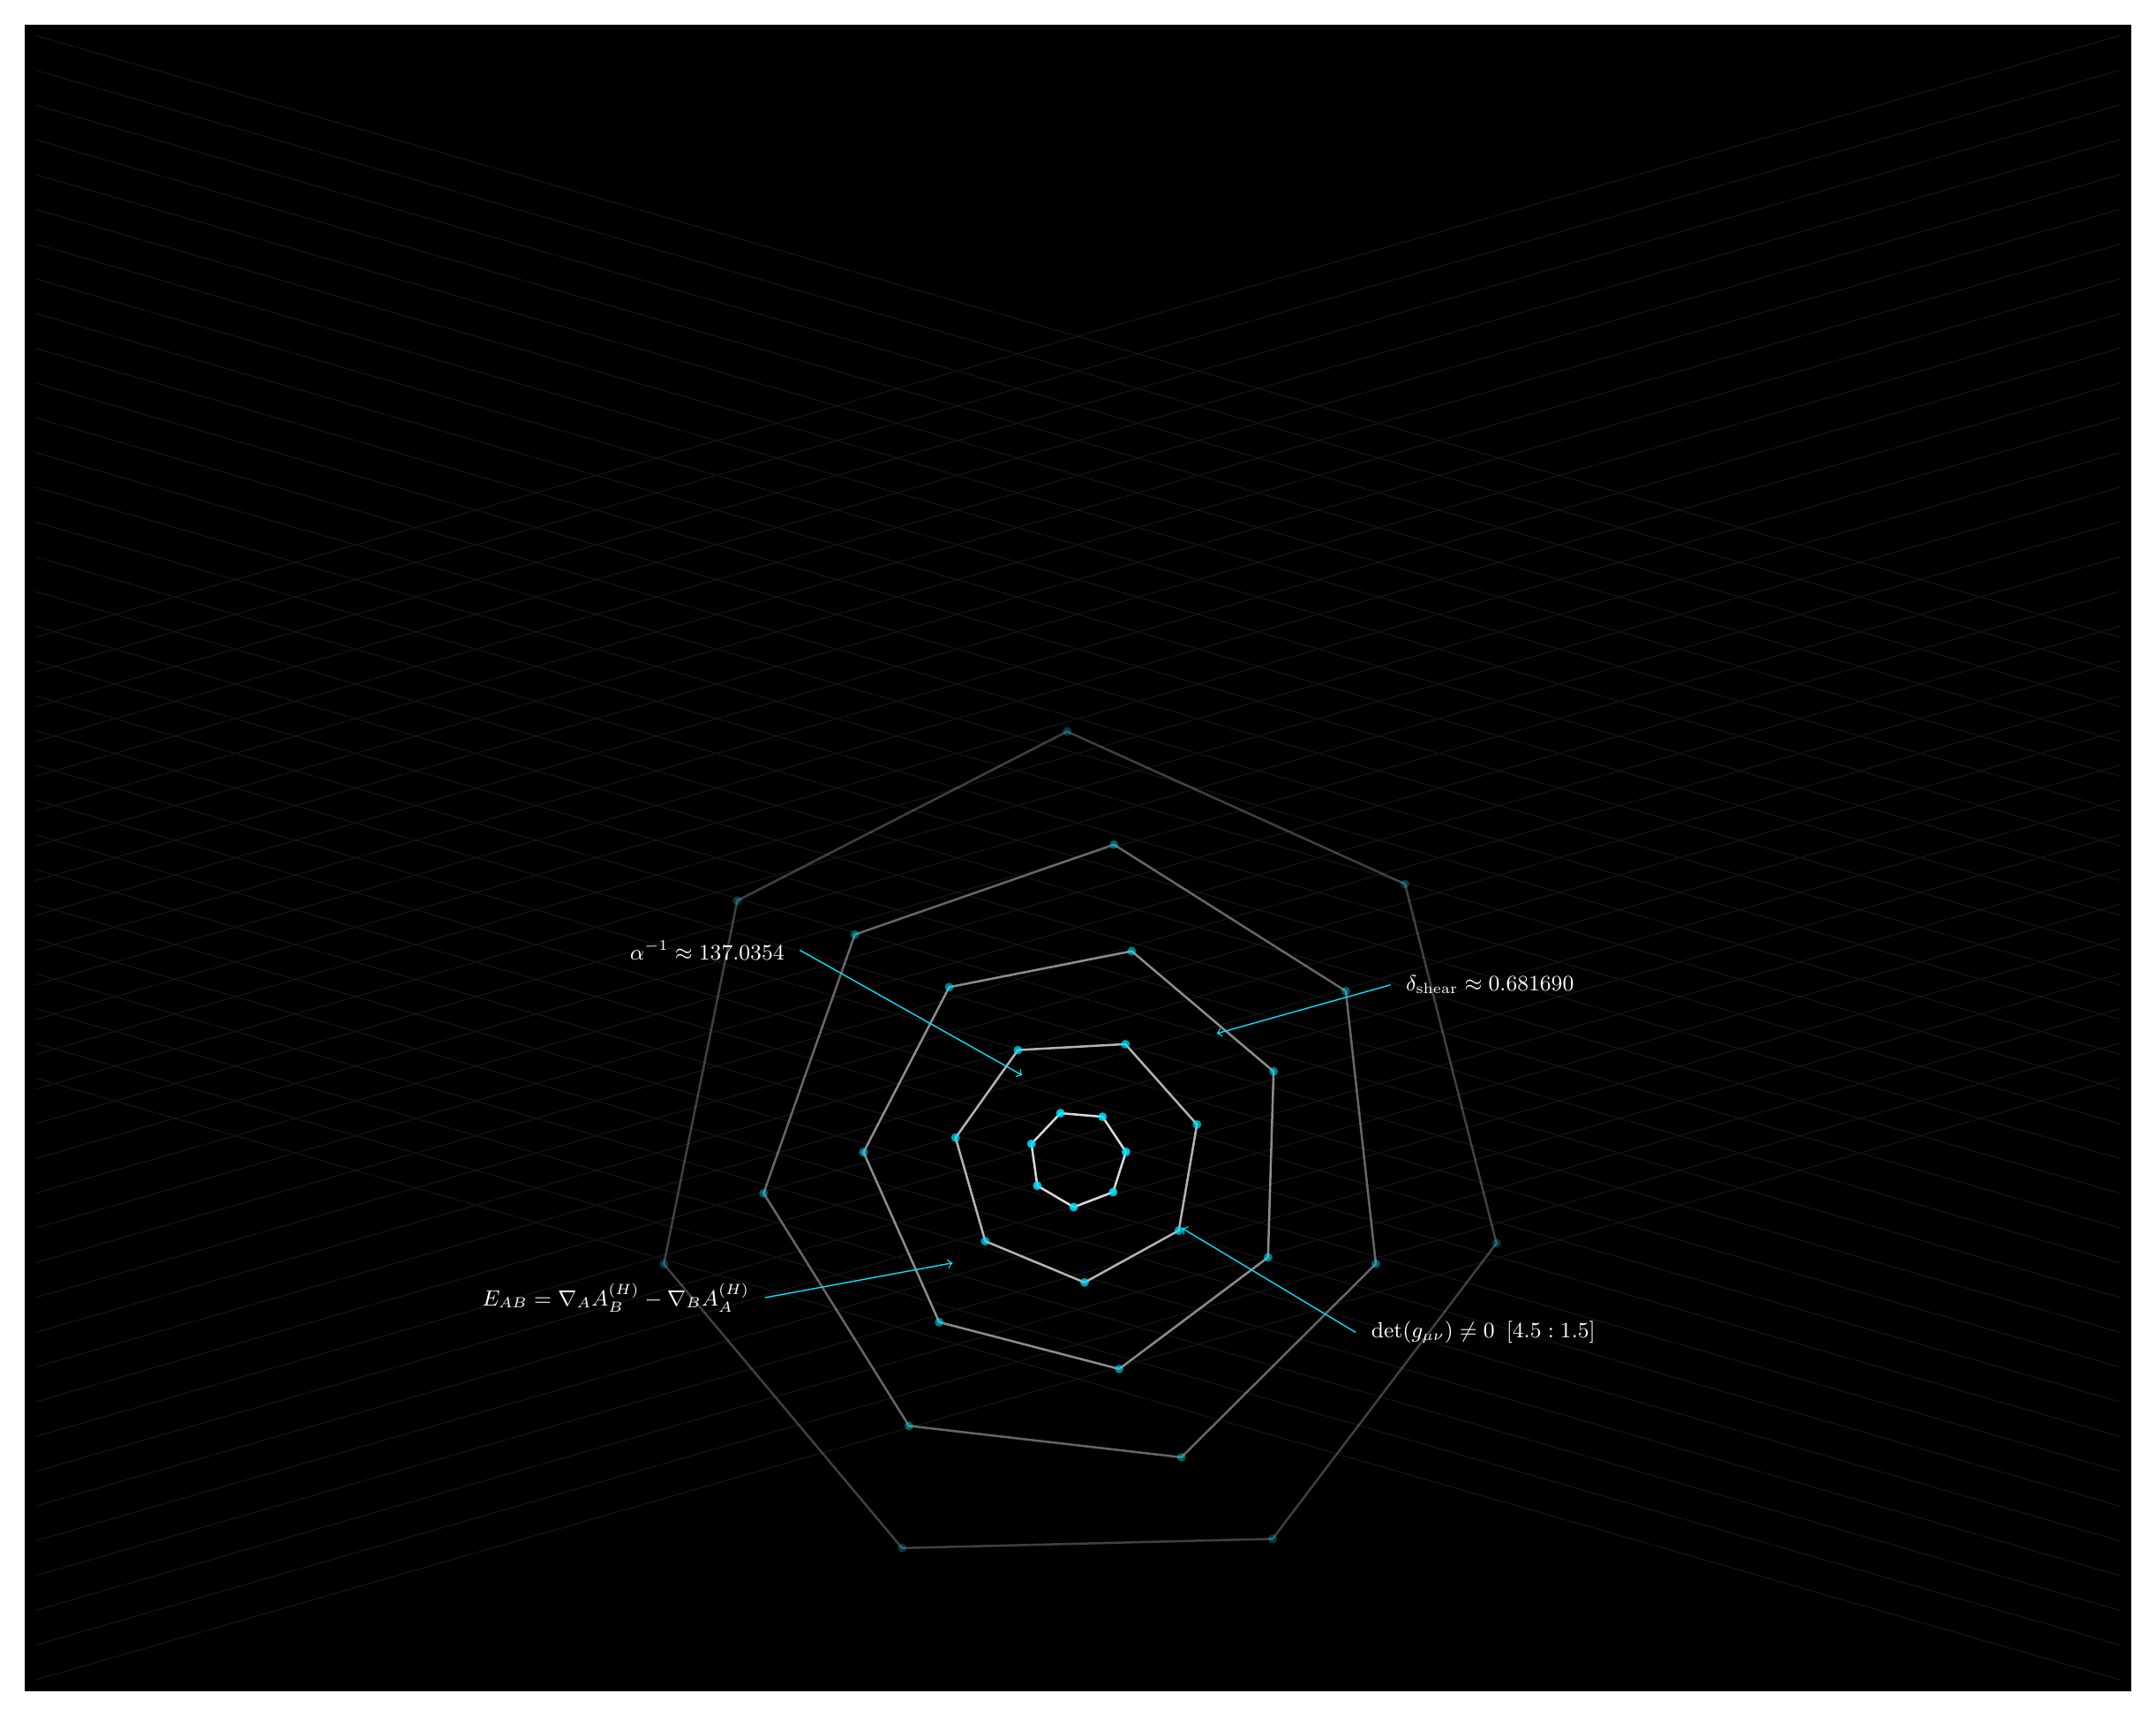
\begin{tikzpicture}[background rectangle/.style={fill=darkbg}, show background rectangle]

    % 1. Isometric Grid Background
    \foreach \i in {-15,-14,...,15} {
        \draw[color=gridline, line width=0.4pt] (-15, \i*0.5) -- (15, \i*0.5 + 8.66);
        \draw[color=gridline, line width=0.4pt] (-15, \i*0.5 + 8.66) -- (15, \i*0.5);
    }

    % 2. Nested, Rotating Heptagons (Unfolding Protocol)
    \foreach \layer in {1,2,3,4,5} {
        \pgfmathsetmacro{\radius}{0.7 * pow(\layer, 1.35)}
        \pgfmathsetmacro{\rotation}{\layer * 8}
        \pgfmathsetmacro{\opacity}{1.0 - (\layer * 0.15)}
        
        % FIX: Explicitly unrolled nodes to eliminate inline path macro errors
        \draw[color=purewhite, opacity=\opacity, line width=0.9pt] 
            (0+\rotation:\radius) -- 
            (51.43+\rotation:\radius) -- 
            (102.86+\rotation:\radius) -- 
            (154.29+\rotation:\radius) -- 
            (205.71+\rotation:\radius) -- 
            (257.14+\rotation:\radius) -- 
            (308.57+\rotation:\radius) -- cycle;
            
        % Overlay Neon Intersections
        \foreach \x in {0, 51.43, 102.86, 154.29, 205.71, 257.14, 308.57} {
            \fill[color=neoncyan, opacity=\opacity] (\x+\rotation:\radius) circle (1.8pt);
        }
    }

    % 3. Structural Pointer Lines & Formula Injections
    \draw[color=neoncyan, line width=0.5pt, ->] (-4, 3) -- (-0.8, 1.2);
    \node[color=purewhite, font=\ttfamily\small, anchor=east] at (-4.1, 3) {$\alpha^{-1} \approx 137.0354$};

    \draw[color=neoncyan, line width=0.5pt, ->] (4, -2.5) -- (1.5, -1.0);
    \node[color=purewhite, font=\ttfamily\small, anchor=west] at (4.1, -2.5) {$\det(g_{\mu\nu}) \neq 0 \ [4.5:1.5]$};

    \draw[color=neoncyan, line width=0.5pt, ->] (-4.5, -2) -- (-1.8, -1.5);
    \node[color=purewhite, font=\ttfamily\small, anchor=east] at (-4.6, -2) {$E_{AB} = \nabla_A A_B^{(H)} - \nabla_B A_A^{(H)}$};

    \draw[color=neoncyan, line width=0.5pt, ->] (4.5, 2.5) -- (2.0, 1.8);
    \node[color=purewhite, font=\ttfamily\small, anchor=west] at (4.6, 2.5) {$\delta_{\mathrm{shear}} \approx 0.681690$};

\end{tikzpicture}
\end{document}
